\documentclass[]{beamer}
\usepackage[T1]{fontenc}
\usepackage[utf8]{inputenc}
\usepackage{lmodern}
\usepackage[italian]{babel}
\usepackage{mathrsfs}
\usepackage{cancel}

\title{La gravitazione}
\author{\texorpdfstring{Mattia Cozzi\newline\href{mailto:cozzimattia@gmail.com}{\texttt{cozzimattia@gmail.com}}}{Mattia Cozzi}}
\date{a.s.~2023/2024}

%\documentclass[handout]{beamer}     %usare questa classe per generare l'handout
%\usepackage{pgfpages}   %per mostrare più quadri nella stessa pagina
%\pgfpagesuselayout{4 on 1}[a4paper,border shrink=5mm,landscape]
\usetheme{Singapore}
%\useoutertheme[left]{sidebar} %elementi intorno alle diapositive
\setbeamercovered{dynamic} %modifica l'aspetto del testo grigetto delle diapositive future. Argomenti: invisible/transparent/dynamic
\usecolortheme{orchid}
%COLORE PRINCIPALE
% \definecolor{marroncino}{RGB}{156, 26, 0} % UBC Blue (primary)
% \setbeamercolor{structure}{fg=marroncino} % itemize, enumerate, etc

\theoremstyle{plain}
\newtheorem{teorema}{Teorema}

\usepackage{tikz}
\usepackage{circuitikz}

\usepackage{pgf,pgfplots,graphicx}
\usetikzlibrary{angles,quotes,arrows,shapes,decorations.markings}
\pgfplotsset{compat=1.15}
\usepgfplotslibrary{units,fillbetween} % to add units easily to axis

\newcommand{\fem}{f_{em}}

\def\angolo[#1](#2)(#3:#4:#5)% Syntax: [draw options] (center) (initial angle:final angle:radius)
    { \draw[#1] ($(#2)+({#5*cos(#3)},{#5*sin(#3)})$) arc (#3:#4:#5); }


\begin{document}

\begin{frame}
  \titlepage
\end{frame}





\begin{frame}
\frametitle{Contenuti}
\tableofcontents
\end{frame}


\section{Keplero}


\begin{frame}
\frametitle{Modello cosmologico}
\begin{columns}
\begin{column}{0.2\textwidth}
\visible<1->{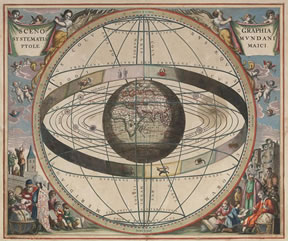
\includegraphics[width=\columnwidth]{img/tolomeo.jpg}}
~
\visible<2->{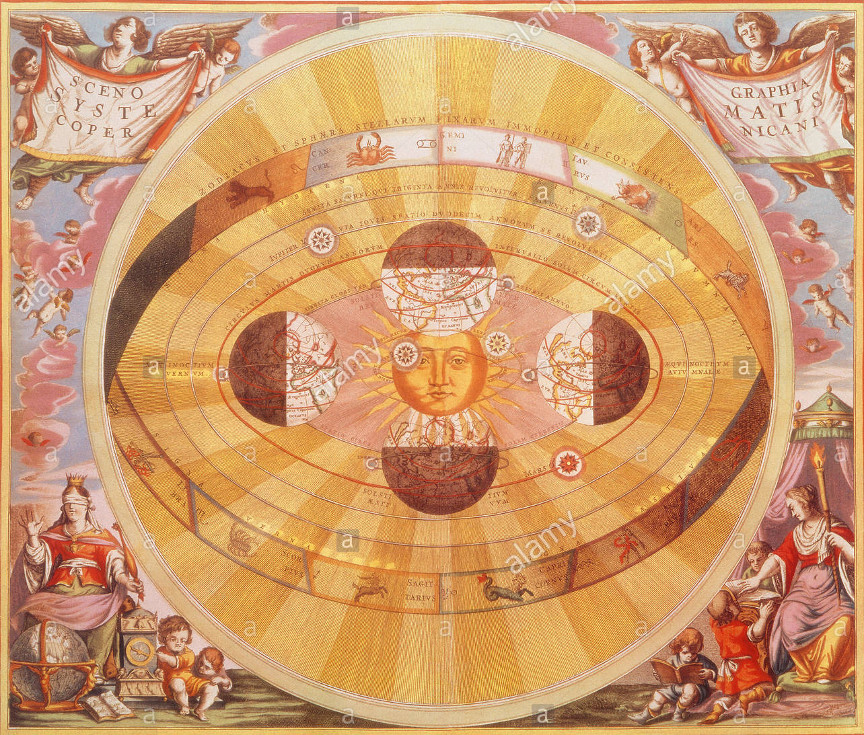
\includegraphics[width=\columnwidth]{img/copernico.jpg}}
~
\visible<3->{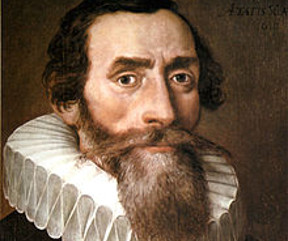
\includegraphics[width=\columnwidth]{img/keplero.jpg}}
\end{column}
\begin{column}{0.6\textwidth}
\begin{itemize}
\item<1-> Tolomeo (150, \emph{Almagesto}) propone un modello \alert<1>{geocentrico} con orbite circolari;
\item<2-> Niccolò Copernico (1543, \emph{De Revolutionibus Orbium Coelestium}) propone un modello \alert<2>{eliocentrico};
\item<3-> Johannes Kepler enuncia le sue \alert<3>{leggi} (1609, \emph{Astronomia Nova});
\item<4-> Isaac Newton propone la \alert<4>{gravitazione universale} (1687, \emph{Philosophiae Naturalis Principia Mathematica}).
\end{itemize}
\end{column}
\end{columns}
\end{frame}

\begin{frame}
\frametitle{Il modello eliocentrico}
Il modello di Copernico fu concepito per ridurre la complessità dei calcoli necessari a predire le posizioni dei pianeti (\emph{rasoio di Occam}?)

~

Prevedeva il Sole al centro ed i pianeti in orbita intorno ad esso, secondo \alert{traiettorie circolari}.

~

Il modello di Copernico non era però perfetto: i calcoli non erano in accordo con le osservazioni astronomiche (molto precise quelle di Tycho Brahe, fine XVI secolo).
\end{frame}

\begin{frame}
\frametitle{Keplero}
Keplero risolse i problemi del modello copernicano proponendo \alert{orbite ellittiche} anziché circolari.
\begin{figure}
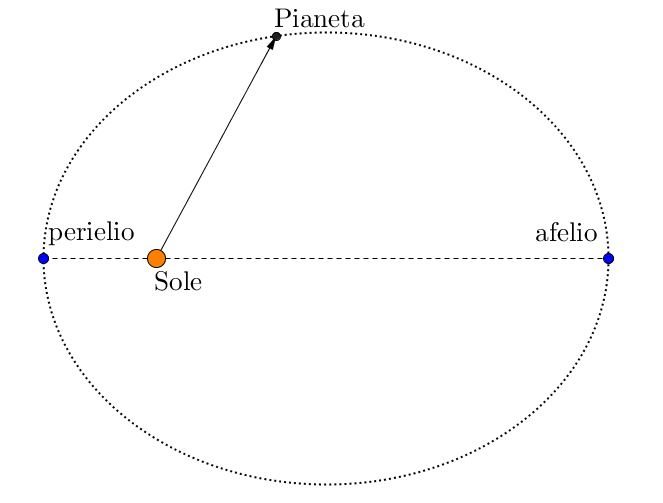
\includegraphics[width=.5\columnwidth]{img/orbitaellittica.jpg}
\end{figure}

\begin{center}
\href{gif/ellisse.gif}{\beamergotobutton{Video: Generazione di un'ellisse}}
\end{center}
\end{frame}


\begin{frame}
\frametitle{La prima legge}
\begin{block}{Prima legge di Keplero}
Le orbite descritte dai pianeti attorno al Sole sono ellissi di cui il Sole occupa uno dei due fuochi.
\end{block}
\begin{center}
\href{gif/keplero1.gif}{\beamergotobutton{GIF: Prima legge}}
\end{center}\pause


Generalmente, l'eccentricità dell'orbita dei pianeti è molto bassa ($ e_{Terra} = 0,017 $) e possiamo spesso approssimare l'orbita come circolare (tuttavia $ e_{Plutone} = 0,244 $).\pause

~

Questa legge vale anche per gli altri oggetti che gravitano intorno al Sole: $ e_{Halley} = 0,967 $.
\end{frame}


\begin{frame}
\frametitle{La seconda legge}
\begin{block}{Seconda legge di Keplero}
Il raggio vettore che va dal Sole ad un pianeta spazza aree uguali in intervalli di tempo uguali.
\end{block}
\begin{figure}
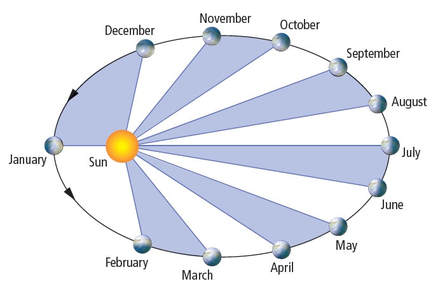
\includegraphics[width=.5\columnwidth]{img/keplero2.jpg}

\href{gif/keplero2.gif}{\beamergotobutton{GIF: Seconda legge}}
\end{figure}\pause
Il pianeta risulta più veloce al perielio e più lento all'afelio.
\end{frame}



\begin{frame}
\frametitle{La terza legge}
\begin{block}{Terza legge di Keplero}
Il rapporto tra il cubo del semiasse maggiore dell'orbita e il quadrato del periodo di rivoluzione è lo stesso per tutti i pianeti.
\begin{center}
\colorbox{blue!30}{$ \dfrac{a^3}{T^2}=k $}
\end{center}
\end{block}\pause

~

Ne risulta che più un pianeta è distante dal Sole, maggiore è il suo periodo di rivoluzione: 
\begin{itemize}
  \item $ a_{Terra} = 1,5 \times 10^{11} \, m $ e $ T_{Terra} = 1 \, anno $;\pause
  \item $ a_{Plutone} = 5,9 \times 10^{12} \, m = $ e $ T_{Plutone} = 249,7 \, anni $.
\end{itemize}
\begin{center}
\href{gif/keplero3.gif}{\beamergotobutton{GIF: Terza legge}}
\end{center}
\end{frame}





\section{Gravitazione universale}






\begin{frame}
\frametitle{Leggi descrittive e leggi causali}
Le leggi di Keplero descrivono ottimamente il moto dei pianeti intorno al Sole, ma non spiegano il \emph{motivo} di tali moti.\pause

~

Newton propose una forza, la \alert{forza di gravità}, per cui due corpi dotati di massa si attraggono.\pause

~

La stessa forza che fa cadere a terra gli oggetti, tiene in orbita i pianeti e i loro satelliti.
\end{frame}



\begin{frame}
\frametitle{La gravitazione universale (1)}
\begin{block}{Legge di gravitazione universale}
La forza di attrazione gravitazionale tra due corpi puntiformi di massa $ m_1 $ e $ m_2 $ a distanza $ r $ è diretta lungo la linea che congiunge i due corpi e ha modulo:
\begin{center}
\colorbox{blue!30}{$ F = G \,  \dfrac{m_1 \, m_2}{r^2} $}
\end{center}
$ G = 6,67 \times 10^{-11} \, \frac{Nm^2}{kg^2}$ =  cost.~di gravitazione universale
\end{block}
\end{frame}

\begin{frame}
\frametitle{La gravitazione universale (2)}
\begin{columns}
\begin{column}{0.3\textwidth}
\begin{center}
\colorbox{blue!30}{$ F = G \,  \dfrac{m_1 \, m_2}{r^2} $}
\end{center}
\end{column}
\begin{column}{0.5\textwidth}
\begin{figure}
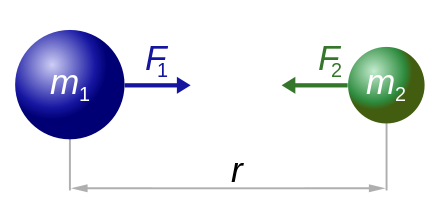
\includegraphics[width=\columnwidth]{img/gravitazione.png}
\end{figure}
\end{column}
\end{columns}\pause

Notiamo che:
\begin{itemize}
  \item se una delle masse raddoppia, la forza di attrazione raddoppia;\pause
  \item se la distanza raddoppia, le forza di attrazione diventa quattro volte meno intensa (non ``sentiamo'' la gravità delle stelle!).
\end{itemize}
\end{frame}


\begin{frame}
\frametitle{Gravitazione universale e leggi di Keplero}
Le tre leggi di Keplero possono essere \alert<1>{dedotte matematicamente} dalla legge di gravitazione universale.\pause

~

La legge di gravitazione universale motiva quindi le tre leggi descrittive di Keplero.
\end{frame}



\begin{frame}
\frametitle{Esercizio}
\begin{exampleblock}{Gravitazione di un satellite artificiale}
  \small{Un satellite di diametro trascurabile orbita intorno alla Terra alla distanza di $ 500 \, km $ dalla superficie terrestre e risente di una forza di $ 3,50 \times 10^{6} \, N $. La massa della Terra vale $ 5,976 \times 10^{24} \, kg $. Trattiamo il problema come se le masse dei corpi fossero tutte concentrate nei loro centri. 

  Quanto vale la massa del satellite?\hspace*{\fill}[$ 4,16 \times 10^{5} \, kg $]}
\end{exampleblock}\pause

~

Ricorda che la distanza tra i due centri di massa è pari alla somma tra il raggio terrestre e l'altitudine dell'orbita.
\end{frame}




\section{Peso}

\begin{frame}
\frametitle{La forza peso (1)}
Vediamo allora con un nuovo occhio una forza che già conosciamo:
\begin{block}{Forza peso}
La forza peso $ \vec{P} $ di un corpo di massa $ m $ è la forza di gravità con cui il pianeta attrae tale massa quando questa è posta sulla superficie del pianeta.
\end{block}\pause
Tendiamo a considerare la forza peso come costante, ma in effetti essa, dipendendo dalla distanza dal centro della Terra, ha una leggera \alert{variazione in funzione dell'altitudine}.
\end{frame}

\begin{frame}
\frametitle{La forza peso (2)}
Essendo $ m $ la massa di un corpo, $ M = 5,98 \times 10^{24} \, kg $ la massa della Terra, $ r = 6 \, 378 \, km $ il raggio della Terra e $ h $ l'altitudine a cui si trova il corpo:
\begin{center}
$ P = G \,  \dfrac{m \, M}{(r+h)^2} ~~~ \Longrightarrow ~~~ mg = m \,  \dfrac{G \, M}{(r+h)^2}  $
\end{center}\pause
\begin{center}
$ g = \dfrac{G \, M}{(r+h)^2} $
\end{center}\pause
\begin{columns}
\begin{column}{0.3\textwidth}
\begin{center}
Mare

$ g_{0 \, m} = 9,81 \, \frac{m}{s^2} $
\end{center}\pause
\end{column}
\begin{column}{0.3\textwidth}
\begin{center}
Everest

$ g_{8848 \, m} = 9,78 \, \frac{m}{s^2} $
\end{center}\pause
\end{column}
\begin{column}{0.3\textwidth}
\begin{center}
ISS

$ g_{408 \, km} = 8,73 \, \frac{m}{s^2} $
\end{center}
\end{column}
\end{columns}
\end{frame}

\begin{frame}
\frametitle{Esercizio}
\begin{exampleblock}{Intensità di $ g $ sulla Luna}
  \small{Sulla Luna l'accelerazione di gravità è circa 1/6 di quella terrestre.

  Calcola la massa della Luna.\hspace*{\fill}[$ 7,40 \times 10^{22} \, kg $]}
\end{exampleblock}
\end{frame}




\begin{frame}
\frametitle{Massa inerziale e massa gravitazionale}
\begin{columns}
\begin{column}{0.45\textwidth}
\begin{center}
$ F = ma $
\end{center}
La \emph{massa inerziale} di un corpo è una misura della resistenza di un corpo ad assere accelerato.\pause
\end{column}
\begin{column}{0.45\textwidth}
\begin{center}
$ F = G \,  \dfrac{m_1 \, m_2}{r^2} $
\end{center}
La \emph{massa gravitazionale} di un corpo misura la sua capacità di attrarre altre masse e di essere attratto da esse.\pause
\end{column}
\end{columns}

~

~

Sono pertanto, in linea di principio, \alert{due concetti distinti}.\pause

~

Misurazioni sperimentali estremamente precise mostrano tuttavia che esse sono \alert{direttamente proporzionali} e pertanto, dal punto di vista pratico, possiamo ignorare tale distinzione (che pure esiste concettualmente). 
\end{frame}


\section{Satelliti}

\begin{frame}
\frametitle{Orbita circolare}
Supponiamo di avere un satellite di massa $ m $ in orbita circolare intorno ad un pianeta a distanza $ R = r + h $.\pause

~

La forza di gravità agisce da \alert<2>{forza centripeta}, e pertanto:
\begin{center}
$ F_G = F_C ~~~ \pause\Longrightarrow ~~~ G\dfrac{mM}{R^2} = m \dfrac{v^2}{R} ~~~ \pause\Longrightarrow ~~~ v = \sqrt{\dfrac{GM}{R}} $
\end{center}\pause
Notiamo che \alert<5>{la velocità dell'orbita non dipende dalla massa del satellite}.\pause

~

Se la velocità è tale per cui il periodo dell'orbita è uguale al periodo di rotazione della Terra, si parla di \alert<6>{satelliti geostazionari}.
\end{frame}


\begin{frame}
\frametitle{Esercizio}
\begin{exampleblock}{Moto di un satellite}
  \small{Un satellite ruota intorno ad un pianeta su un'orbita circolare di raggio $ 1,741 \times 10^{6} \, m $. La sua velocità di valore costante è $ 1,6 \times 10^{3} \, m/s $.

  Quanto vale la massa del pianeta?\hspace*{\fill}[$ 6,7 \times 10^{22} \, kg $]}
\end{exampleblock}
\end{frame}



\begin{frame}
\frametitle{Velocità di fuga}
\begin{block}{Velocità di fuga}
La velocità di fuga è la minima velocità che deve essere posseduta da un proiettile posto sulla superficie di un pianeta per riuscire ad allontanarsi per sempre da esso, senza mai più ricadervi.
\begin{center}
\colorbox{blue!30}{$ v_f = \sqrt{\dfrac{2GM}{R}} $}
\end{center}
\end{block}\pause
Se $ v_f > c $ allora abbiamo un \emph{buco nero}. Il raggio per cui un oggetto di massa $ M $ diventa un buco nero è il \emph{raggio di Schwarzschild}.
\begin{center}
$ R_S = \dfrac{2GM}{c^2} $
\end{center}
\end{frame}

\section{Campo gravitazionale}

\begin{frame}
\frametitle{Il concetto di campo (1)}
La forza tra due masse è una \emph{forza a distanza}.

~

Come possono due corpi non in contatto interagire tra loro?\pause

~

Questa difficoltà viene superata ipotizzando che:
\begin{itemize}
  \item la presenza di una massa in un certo punto dello spazio \alert<2>{modifica le caratteristiche dello spazio} circostante;\pause
  \item un'altra massa posta nello spazio circostante \alert<3>{risente di una forza dovuta alle nuove proprietà dello spazio}.
\end{itemize}
\end{frame}


\begin{frame}
\frametitle{Il concetto di campo (2)}

\begin{figure}
\begin{tikzpicture}[scale=0.5]
\node [above,teal] at (6,.1) {$ m_p $};
\draw [teal, ultra thick,fill=teal] (6,0) circle [radius=.1];\pause
\visible<2->{\draw [->, thick] (6,0) -- (2,0);
\node [above] at (4,0) {$ \vec{F} $};
\node [above,teal] at (0,.7) {$ M $};
\draw [teal, ultra thick,fill=teal] (0,0) circle [radius=.7];
\draw [teal, ultra thick,fill=teal] (6,0) circle [radius=.1];}
\end{tikzpicture}
\end{figure}
Poniamo una \emph<1>{massa di prova} (sufficientemente piccola da non modificare il sistema fisico in esame) $ m_p $ in un punto dello spazio.

~

\visible<2->{Se introduciamo una massa sorgente di campo gravitazionale $ M $ allora \alert{$ m_p $ inizierà a sentire una forza $ \vec{F} $} dovuta alle nuove proprietà del punto in cui si trova.}
\end{frame}


\begin{frame}
\frametitle{Campo vettoriale}
Il campo gravitazionale è un \emph{campo vettoriale}.

\begin{block}{Definizione}
\begin{columns}
\begin{column}{0.4\textwidth}
Un campo vettoriale è una funzione che ad ogni punto dello spazio associa un vettore forza.
\end{column}
\begin{column}{0.4\textwidth}
\begin{figure}
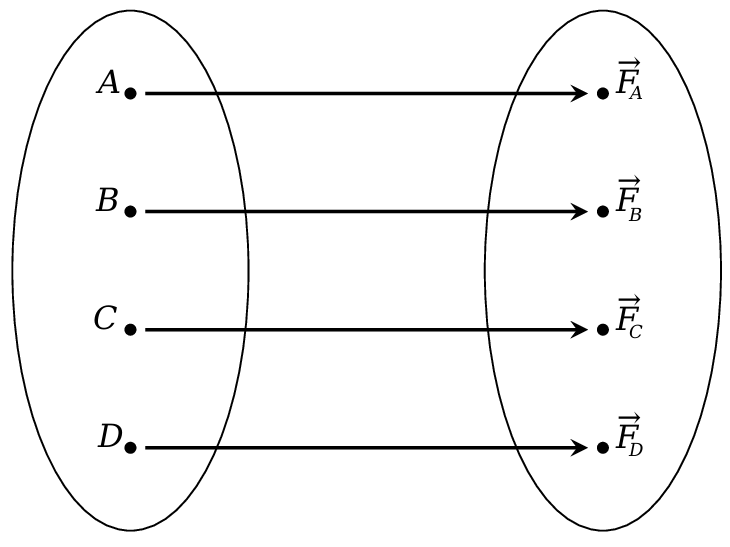
\includegraphics[width=.9\columnwidth]{img/funzionecampo.png}
\end{figure}
\end{column}
\end{columns}
\end{block}

Il vettore forza viene ottenuto con la legge di gravitazione universale.
\end{frame}



\begin{frame}
\frametitle{Il vettore campo gravitazionale}
\begin{figure}
\begin{tikzpicture}[scale=0.5]
\node [above,teal] at (6,.1) {$ m_p $};
\draw [->, thick] (6,0) -- (2,0);
\node [above] at (4,0) {$ \vec{F} $};
\node [above,teal] at (0,.7) {$ M $};
\draw [teal, ultra thick,fill=teal] (0,0) circle [radius=.7];
\draw [teal, ultra thick,fill=teal] (6,0) circle [radius=.1];
\end{tikzpicture}
\end{figure}
Usando la nostra massa di prova $ m_p $ definiamo, per ogni punto dello spazio, il \alert{vettore campo gravitazionale}:

\begin{center}
\colorbox{blue!30}{$ \vec{g} = \dfrac{\vec{F}}{m_p} $}~~~~~~~~$ \left[\dfrac{N}{kg}\right] = \left[\dfrac{m}{s^2}\right]  $
\end{center}\pause
Notiamo che, in ogni punto dello spazio, \alert{$ \vec{g} $ è un vettore}:
\begin{itemize}
  \item con la stessa direzione e lo stesso verso di $ \vec{F} $;\pause
  \item con modulo pari a $ g = \dfrac{F}{m_p} $.
\end{itemize}
\end{frame}


\begin{frame}
\frametitle{Campo di una massa puntiforme}
In ogni punto dello spazio, possiamo calcolare il valore del campo gravitazionale generato da una massa $ M $:
\begin{center}
$ g = \dfrac{F}{m_p} = \dfrac{G \dfrac{M \cancel{m_p}}{r^2}}{\cancel{m_p}} = G \dfrac{M}{r^2} $
\end{center}\pause
In un punto a distanza $ r $, una massa $ M $ genera un campo di intensità:
\begin{center}
\colorbox{blue!30}{$ g = G \dfrac{M}{r^2} $}
\end{center}
\end{frame}





\begin{frame}
\frametitle{Le linee del campo gravitazionale}

\begin{columns}
\begin{column}{0.6\textwidth}
Un campo gravitazionale è costituito da infiniti vettori.

~

Per visualizzarlo introduciamo le \emph{linee del campo gravitazionale}, che saranno:
\begin{itemize}
  \item rivolte verso la massa che genera il campo;
  \item più dense dove il campo è più intenso.
\end{itemize}
\end{column}
\begin{column}{0.3\textwidth}
\begin{figure}
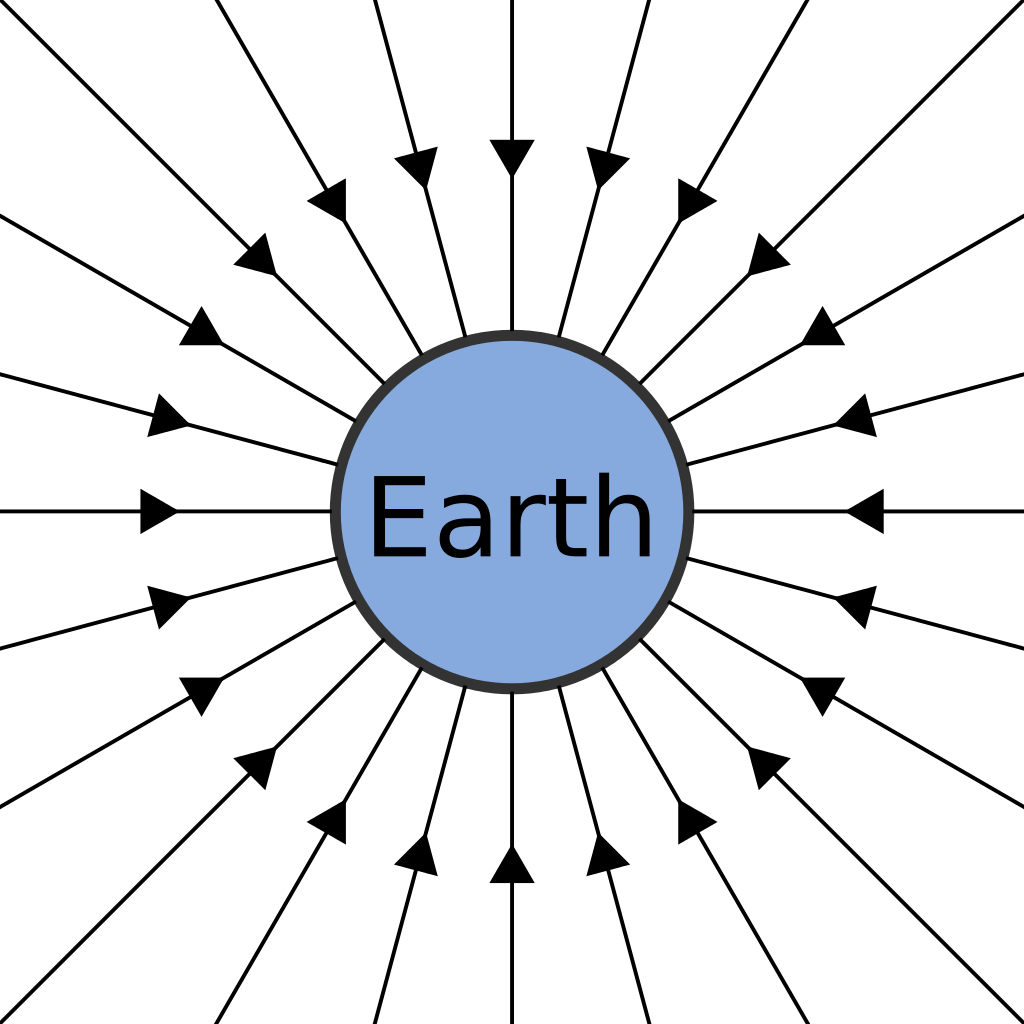
\includegraphics[width=\columnwidth]{img/campograv.png}
\end{figure}
\end{column}
\end{columns}
\end{frame}


\begin{frame}
\frametitle{Esercizio}
\begin{exampleblock}{Intensità del campo gravitazionale}
  \small{Quale raggio dovrebbe avere la Terra affinché il valore del suo campo gravitazionale risulti uguale a quello di Giove?

  Dati: $ m_{G} = 1900 \times 10^{24} \, kg $, $ r_G = 71,4 \times 10^{6} \, m $.\hspace*{\fill}[$ 4,00 \times 10^{6} \, m $]}
\end{exampleblock}
\end{frame}


%slide sulle onde gravitazionali, perturbazioni del campo che viaggiano a velocità c


\end{document}
